\chapter{The Pacific Ocean Neutrino Explorer}

The  Pacific Ocean Neutrino Explorer (P--ONE) is a proposed neutrino telescope planned to operate in the Pacific Ocean near the West Coast of Vancouver Island, Canada \cite{pone}. As with other neutrino telescopes, P--ONE aims to detect and characterize extremely high energy astrophysical neutrinos from galactic and extra--galactic sources \cite{pone}. In particular, due to the planned multi--cubic kilometer coverage, it would be suitable for neutrinos from sources such as Blazars \cite{icecube_nat}. Moreover P--ONE hopes to provide an avenue for research in exotic particle searches, dark matter, neutrino oscillations, supernova neutrinos, and tau neutrino studies ($\nu_{\tau}$) \cite{pone}. 

\section{Geometry}

The geometry of the detector is incredibly important, as the layout and positions of the detectors can drastically change the results and the sensitivies \cite{icecube}. The first proposed Explorer phase for P--ONE corresponds to the first 10 string--segment to be deployed \cite{pone}. Each string will be composed of 20 photo--sensors and at least two calibration modules \cite{pone}, with the strings organized in an array similar to that of IceCube \cite{pone,icecube}. In order to avoid using thousands of strings to get a larger coverage, it can achieve a similar amount of information using a segmented approach where six more arrays similar to those of the Explorer are added around it \cite{pone}. This design is drawn in Figure \ref{fig:pone_geo}. 

\begin{figure}[h]
  \centering
  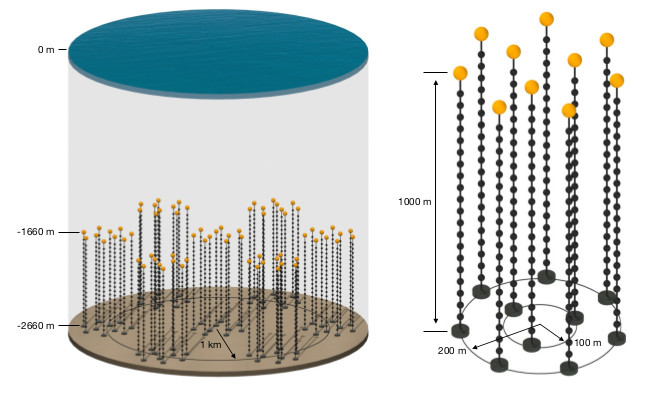
\includegraphics[width=12cm]{./Figures/PONEv0_-23_design.jpg}
  \caption{Left: Proposed full detector of the P--ONE detector. Right: Proposed array for the Explorer deployment of P--ONE.}
  \label{fig:pone_geo}
\end{figure}

With the current proposed geometry, the detector will be incredibly sensitive to horizontal incoming high energy muons from astrophysical neutrino sources \cite{pone}. 

\section{Detectors}
Similar to previously constructed neutrino telescopes, P--ONE will primarily use Vavilov--Cherenkov Radiation from leptons produced through neutrino interactions. This electromagnetic radiation is then detected through highly sensitive optical modules containing photomultiplier tubes (PMTs).

\subsection{Photomultiplier Tubes}

A key part of any neutrino telescope is the detection mechanism, and in this community the PMT is synonomous with detector. The PMT is a vacuum--sealed photocathode with dynode and anodes above connector pins \cite{ham}. The primary mechanism of a PMT is the photoelectric effect from a photon hitting the photocathode \cite{pmt_hist}. This ejected electron than travels and collides with another cathode, which results in more elctrons being ejected. This results in a cascade of electron showers along the dynodes and anodes amplifying the signal before it reaches the connector pins \cite{pmt_hist}. Through this method the PMT can produce large signals at the single photon level, yet is only sensitive to a particular range of frequencies/wavelengths of light \cite{pmt_hist}.

In particular, PMTs are generally sensitive to wavelengths anywhere as low as 100 nm to as high as 500 nm depending on the material of the photochathode \cite{ham}. Another property of PMTs to note is the Quantum Efficiency (QE), which is defined as the ratio of photoelectrons emitted by the photocathode to the number of incident photons \cite{ham}. Thus, QE defines the probability an incident photon causes a signal. The QE is dependent upon the photocathode and varies with the incident photons wavelength, as different wavelengths carry different energies \cite{ham}.

In contrast to QE, the Dark Current (Dark Noise) is the reporting by PMTs of light even in completely dark environments \cite{ham}. According to the Hamamatsu handbook \cite{ham}, a number of reasons can be the cause for this misfiring in PMTs including (but not limited to) thermionic emissons, internal current leakage, scintillation from glass envelope and radiation sources. One can minimize the effect from these sources, such as reducing the temperature to limit the thermionic emissions \cite{ham}.

The final aspect of PMTs we discuss is afterpulsing, the small pulses observed after the arrival of a signal \cite{ham}. The quick afterpulses (within nano--seconds) can usually be attributed to scattering of electrons on the first dynode \cite{ham}, while later afterpulses (within microseconds) can be the result of positive ions from the ionization of residual gases in the tube \cite{ham}.

The PMT is an incredibly technical piece of hardware, and characterizing each PMT is important to understanding the detector as a whole. 

\subsection{Digital Optical Modules}

In IceCube, the Digitial Optical Module (DOM) is a module containing a ten--inch PMT supported by coupling gel, the high voltage generator, an LED flasher board for calibration, and the mainboard used for analog and digital signal processing \cite{icecube_pmt,icecube} which allows for near--autonomous function. P--ONE will be adopting this approach for detector construction.

\begin{figure}[H]
  \centering
  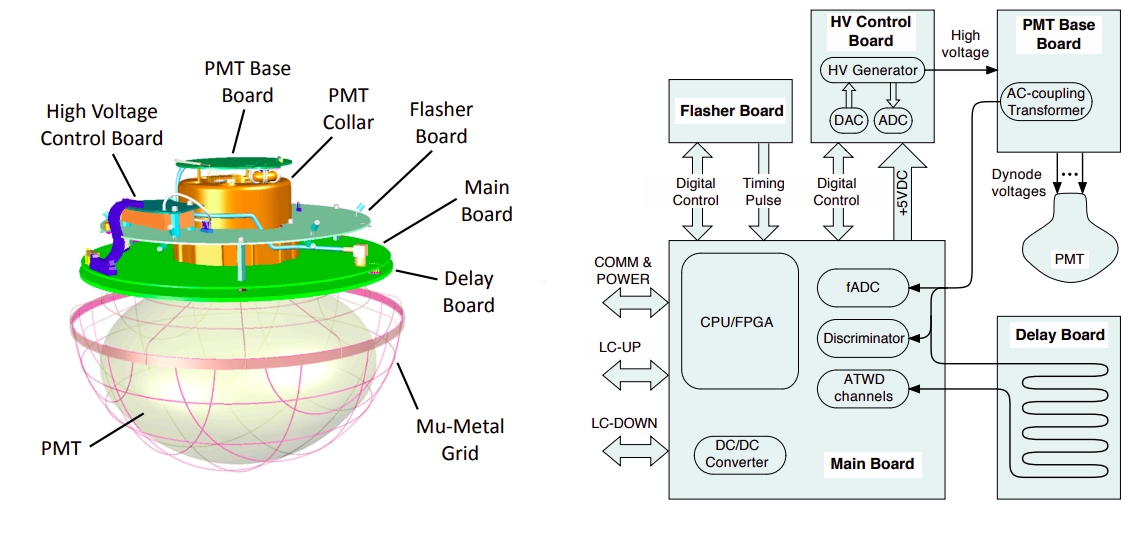
\includegraphics[width=.9\textwidth]{./Figures/icecube_dom.png}
  \caption{A diagram and schematic of the IceCube DOM.}
  \label{fig:ice_dom}
\end{figure}

Figure \ref{fig:ice_dom} shows a diagram of the IceCube DOM along with a schematic of the electronics that are on board. 


\subsection{mDOMs}

A proposed redesign of the IceCube DOM to increase the granularity of light detection is the multi--DOM (mDOM). In place of one large PMT, multiple smaller PMTs can line the same space and provide coverage at the cost of gaps between detectors. The benefit being that individual hits on the smaller PMTs can provide extra information using the acceptance angle and directionality of that particular PMT \cite{mpmt}. Moreover, in theory this can also reproduce the standard DOM data as the signal collected by a single PMT in the array can be collected and treated as a hit for the entire DOM. This gives the mDOMs a felxibility that isn't present for standard DOMs. In IceCube the standard DOMs use a ten--inch diameter PMTs \cite{icecube}, where the mDOMs would use up to 24 three--inch diameter PMTs \cite{mpmt}.

\section{Strings for Absorption length in Water}

The Pathfinder mission for P--ONE is the STRings for Absroption length in Water (STRAW) and its follow up STRAW--b, which were deployed in 2018 and 2020 respectively. The purpose of these missions was to test the technical details of running an experiment like P--ONE, such as the hardware limitation, to provide data to measure the Attenuation length of light in water for light in wavelengths between 350 nm and 600 nm, characterize the bioluminescence of deap--sea living organisms and the $^{40}$K dissolved in the salty water \cite{straw}.

\begin{figure}[H]
  \centering
  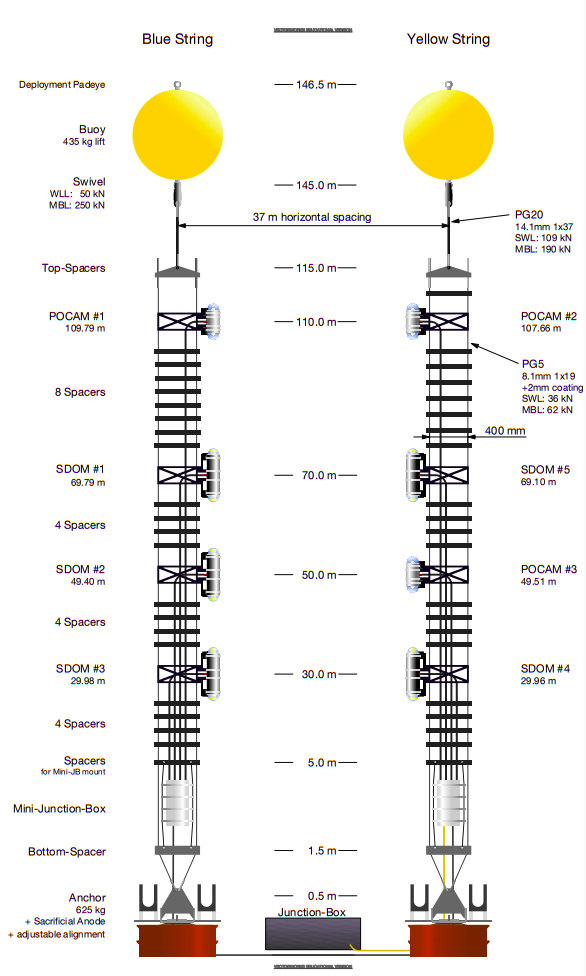
\includegraphics[width=.7\textwidth]{./Figures/STRAW.png}
  \caption{A diagram of the full STRAW setup including distances \cite{straw}.}
  \label{fig:straw}
\end{figure}

The basic design of STRAW, as shown in Figure \ref{fig:straw}, is the same as that of standard Neutrino Telescopes; using PMTs for detecting photons and calibrating light emmitting sources on mooring lines to collect data \cite{straw}. In this particular case STRAW uses two vertical mooring lines with $3^{\prime\prime}$ PMTs and Precision Optical Calibration Modules (POCAMs) for the calibration sources \cite{straw}, which provide isotropic and short pulsed flashes of light. The attenuation length $L_{T}$ in water can be realized using the known photon intensity $N_{0}$, the wavelength from the POCAM flashes and the distance $r$ to each particular PMT with effective collection area $A_{\text{det}}$ measuring an intensity $N(r)$ \cite{straw}. This yields
\begin{equation}
  N(r) = \frac{N_{0}}{4\pi r^{2}}\exp\left(-\frac{r}{L_{T}}\right)A_{\text{det}}\, .
\end{equation}
The expected maximum value of absorption length is around 50 meters, so the STRAW geometry has been chosen to cover the ranges between 20 m and 90 m \cite{straw}. Some of the geometry choices were purely due to technical limitations, such as the maximum safe cable lengths to minimize data loss \cite{straw}, while others were to preserve some form of symmetry between modules \cite{straw}.

Should I talk about POCAMs in detail? \cite{pocam}

\section{Ocean Networks Canada}

The construction and implementation of P--ONE is supported by Ocean Networks Canada (ONC), an oceanography observatory with a vast network monitoring the west and east coasts of Canada along with the arctic \cite{onc}. Situated at the University of Victoria, ONC uses cabled observatories, remote control systems and interactive sensors for data collection and evidence--based decision--making \cite{onc}. 

\begin{figure}[h]
  \centering
  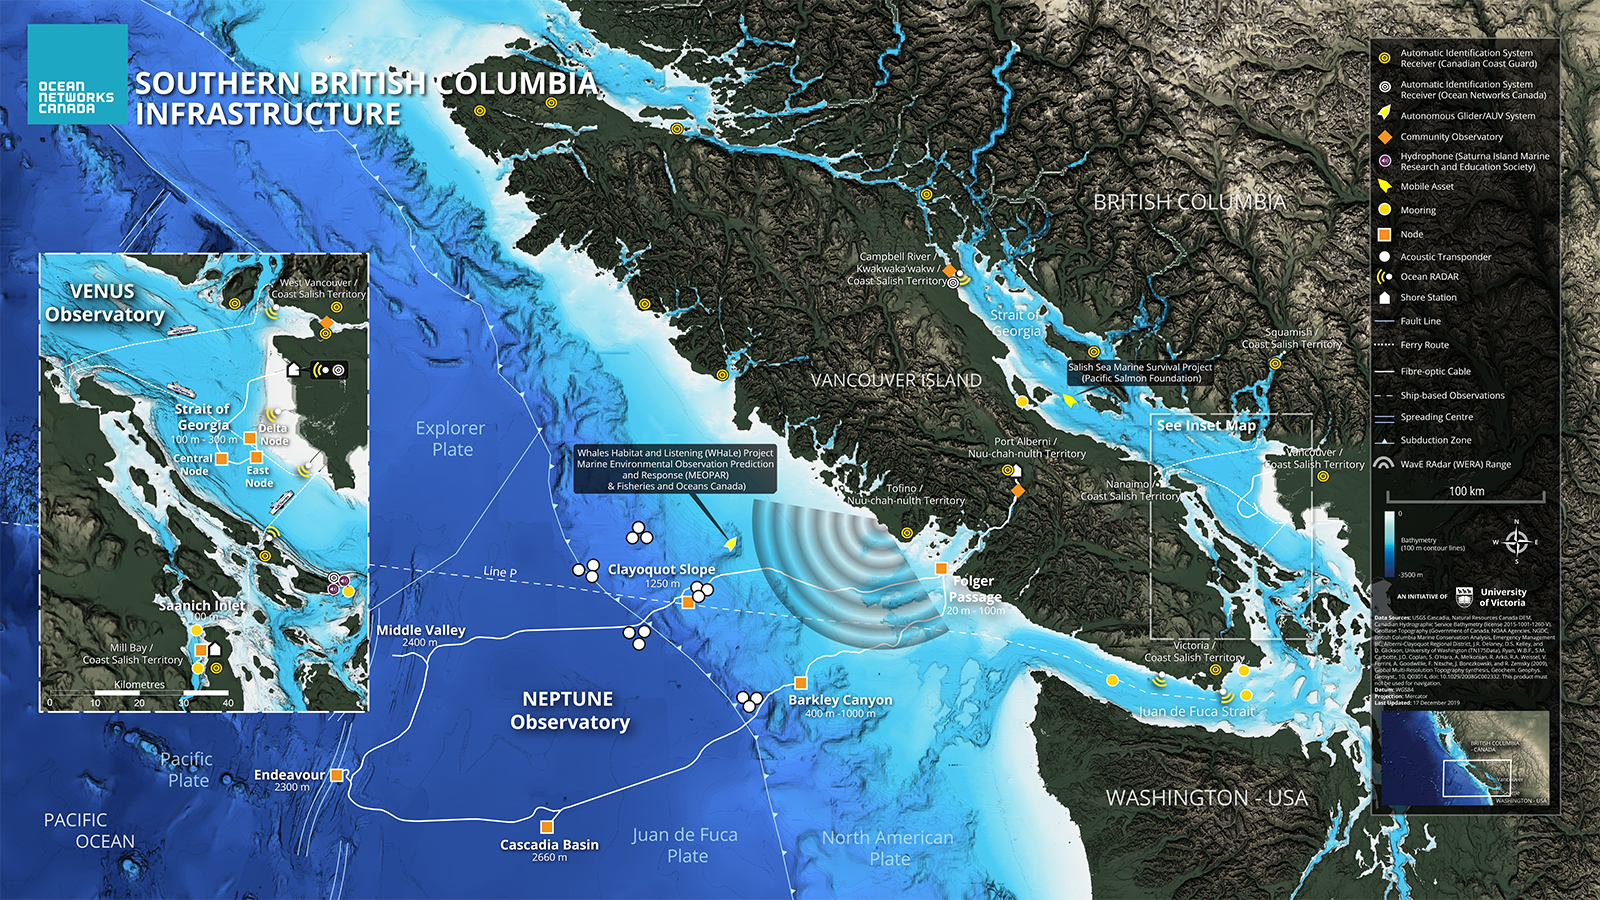
\includegraphics[width=.9\textwidth]{./Figures/western_infrastructure.png}
  \caption{A diagram of the Ocean Networks Canada Western Infrastructure for monitoring the Pacific Ocean. This contains the NEPTUNE and VENUS observatories. Source \cite{onc}.}
  \label{fig:west_inf}
\end{figure}

The west coast observatory, as seen in Figure \ref{fig:west_inf}, is comprised of the 800--km NEPTUNE observatory and the nearly 50--km VENUS observatory \cite{onc}, with the NEPTUNE observatory housing the proposed site of P--ONE at the Cascadia Basin. The Cascadia Basin, as seen in Figure \ref{fig:casc}, is a heavily sedimented abyssal plain located 2660 meters below sea level \cite{onc}. Though the environment seems inhospitable, with temperatures below 2$^{\text{o}}$, high--pressure, and a distinct lack of light, one can still find organisms highly adapted to the extreme environment \cite{onc}. 

\begin{figure}
  \centering
  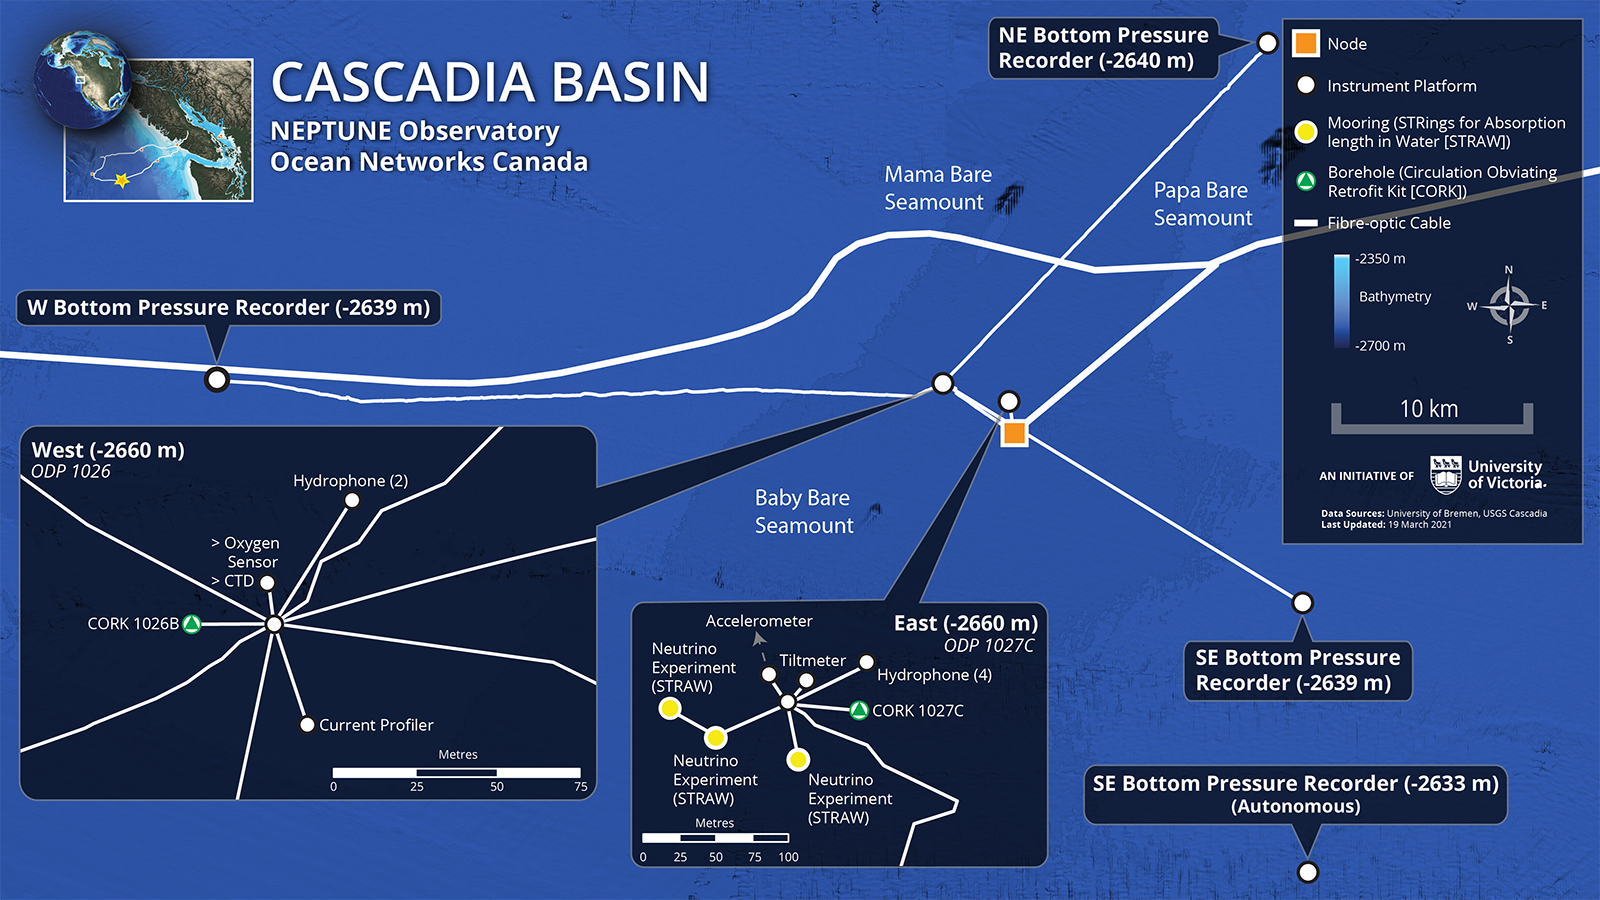
\includegraphics[width=.9\textwidth]{./Figures/cascadia_basin.png}
  \caption{Diagram of the Cascadia Basin, the site of the upcoming P--ONE experiment and current site of the pathfinder STRAW. Source \cite{onc}.}
  \label{fig:casc}
\end{figure}

This biodiversity results in the potential background of bioluminescence \cite{pone,onc,biolum,biolum_rec}. Bioluminesence is the emission of visible light by living organisms due to natural chemical processes used by a wide range of species \cite{biolum}. Some studies show that 75\% of all organisms larger than 1 cm occurring between the surface down to 4000 m depth are capable of bioluminescence \cite{biolum_rec}. Due to evolutionary advantages, most bioluminescent organisms emit light between 440 nm and 540 nm, which also has the largest absorption length in water \cite{biolum}. The amount of photons emitted can also vary significantly from $10^{3}$ for bacterium to $10^{12}$ photons from some fish \cite{biolum}. There are efforts being put together to understand and characterize this background in order to be better prepared for when the detector is installed.



